\documentclass[pdftex,12pt,a4paper]{report}

\usepackage[portuguese,english]{babel}
\usepackage[T1]{fontenc} 
\usepackage[utf8]{inputenc}
\usepackage[pdftex]{graphicx}
\usepackage{minitoc}
\usepackage{hyperref}
\usepackage{indentfirst}
\usepackage[compact]{titlesec}
\usepackage{fancyhdr}
\usepackage{caption}
\usepackage{pgfplots}
\usepackage{pgfplotstable}
\usepackage{fixltx2e}
\usepackage{mathtools}
\usepackage{fancyhdr}
\usepackage{listings}
\usepackage{color}
\usepackage{sverb}
\usepackage[section]{placeins}
\titleformat*{\subsubsection}{\itshape}


%Highlight
\newcommand{\shellcmd}[1]{\indent\indent\texttt{\footnotesize\# #1}\\}

\pagestyle{fancy}
\renewcommand*\thesection{\thechapter\arabic{section}}
\newcommand{\HRule}{\rule{\linewidth}{0.5mm}}
\begin{document}

\begin{titlepage}

\begin{center}


\includegraphics[width=0.15\textwidth]{./logo}\\[0.5cm]    

\textsc{\large Universidade de Aveiro \\[1cm]\large departamento de electrónica, telecomunicações e informática}\\[1cm]

\textsc{\large{1}\large - Desempenho e Dimensionamento de Redes\\[1cm]}

\HRule \\[0.5cm]
{ \huge \bfseries abs}\\[0.4cm]
{ \large \bfseries x}\\[0.4cm]
\HRule \\[1cm]

\textsc{\small{8240 - MESTRADO INTEGRADO EM ENGENHARIA DE COMPUTADORES E TELEMÁTICA}}\\[1cm]

\begin{minipage}{0.4\textwidth}

\begin{flushleft} \large
\href{mailto:rafael.ferreira@ua.pt}{António Rafael da \\ Costa Ferreira }
 \small{\\NMec: 67405}
\end{flushleft}
\end{minipage}
\begin{minipage}{0.4\textwidth}

\begin{flushright} \large
\href{mailto:rodrigocunha@ua.pt}{Rodrigo Lopes \\ da Cunha}
\small{\\NMec: 67800}
\end{flushright}
\end{minipage}\\[1cm]

{\large Docente: Paulo Salvador }\\[0.5cm]

\vfill

{\large Fevereiro de 2016 \\ 2015-2016}

\end{center}

\end{titlepage} %Titulo do Relatorio
\renewcommand{\headrulewidth}{0pt}

%Cabeçalhos de rodapé
\fancyhead{}
\fancyfoot{}
\lhead{Network Statistical Analysis}
\rhead{DDR - 2015/2016}
\lfoot{Rafael Ferreira nmec: 67405 \\ Rodrigo Cunha nmec: 67800}
\rfoot{\thepage}

%Renomear Comandos
\renewcommand*\contentsname{Conteúdos}
\renewcommand*\figurename{Figura}
\renewcommand*\tablename{Tabela}

%Conteúdos, dar paragrafo
\tableofcontents
%Headers
\renewcommand{\headrulewidth}{0.15pt}
\renewcommand{\thechapter}{}

\clearpage

\section{Metrics}
\subsection{Exercício 1}
\subsubsection{codeFiles/metrics.py}
Neste primeiro exercício, era pedido apenas para se analisar os tipos de perfis existentes. Os perfis que foram dados pelos professores no ficheiro \textit{data1}, estão divididos em dois grupos, os primeiros 20 utilizadores com um tráfego mais periódico e os restantes com um tráfego mais irregular, tal como podemos verificar na imagem seguinte:

\begin{figure}[!htb]
\center
 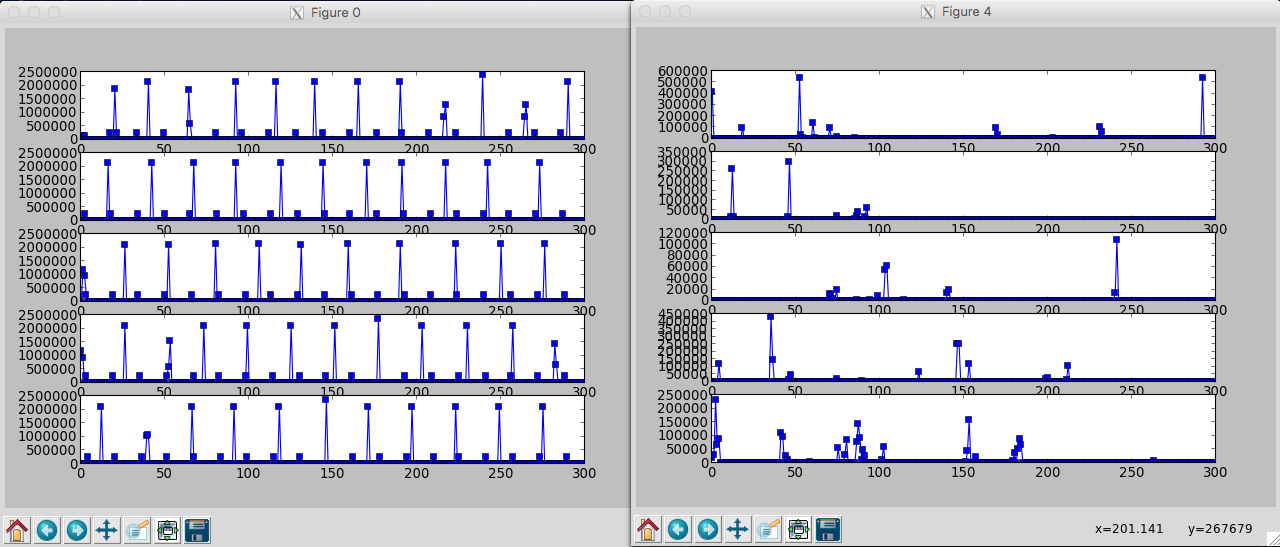
\includegraphics[width=150mm,scale=1]{metrics/typesOfServices.png}
 \caption{Tipos de Perfis dos utilizadores}
 \label{fig:typeOfServices}
\end{figure}

Foi também pedido que se fizesse a representação do nosso perfil, obtido no guia passado, quando se receberam os pacotes do YouTube. O perfil que se obteve \ref{fig:profile}, enquadra num dos dois tipos de perfis acima mostrados.

\begin{figure}[!htb]
\center
 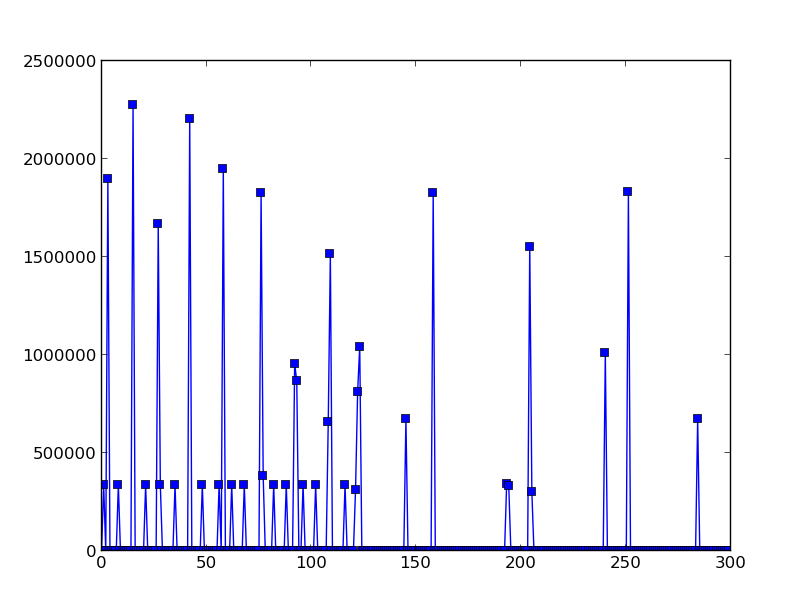
\includegraphics[width=100mm,scale=1]{metrics/profile.png}
 \caption{Perfil obtido}
 \label{fig:profile}
\end{figure}

É possível então verificar que o perfil obtido, se integra no grupo dos 20 primeiros perfis, tendo um tráfego mais periódico que os restantes.

\newpage
\subsection{Exercício 2 e Exercício 3}
\subsubsection{codeFiles/metrics.py (linha 60)}

No 2º exercício, foi pedido que se calculassem valores, como por exemplo a média, a variância, entre outros, para todos os perfis, incluindo o que foi obtido no guia anterior. Com estes valores prentende-se saber qual o tipo de perfil foi obtido. O ficheiro usado para o exercício 2 e 3 é o \textit{metrics.py}.

\begin{figure}[!htb]
\center
 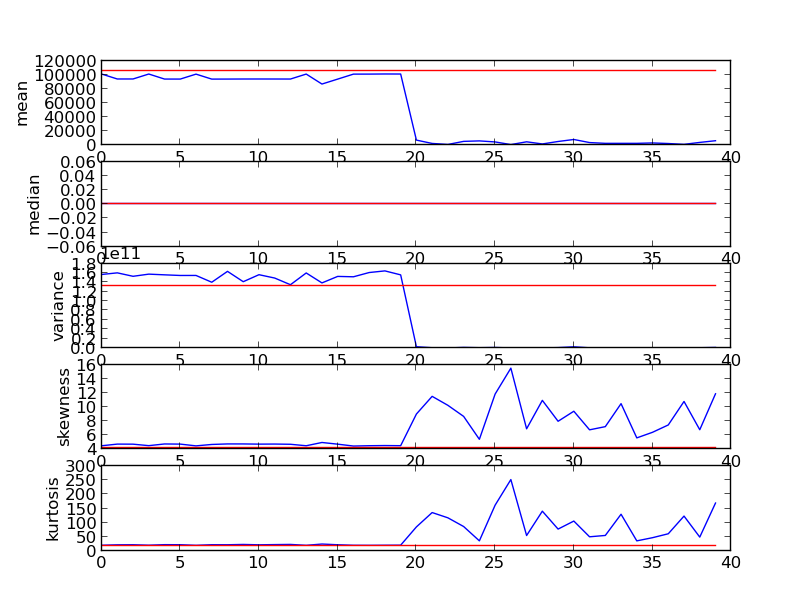
\includegraphics[width=100mm,scale=1]{metrics/compare_profile.png}
 \caption{Comparação de Perfis}
 \label{fig:compare_profile}
\end{figure}

É possível verificar que realmente o perfil obtido, se enquadra no conjunto dos 20 primeiros perfis do ficheiro \textit{data1}, onde o burst de pacotes é mais periódico.

\section{Probability Density Functions (PDF) and Comulative Distribution Function (CDF)}
\subsection{Exercício 4}
\subsubsection{codeFiles/pdf\_cdf.py (linha 41)}


\begin{figure}[!htb]
  \centering
  \begin{minipage}[b]{0.4\textwidth}
    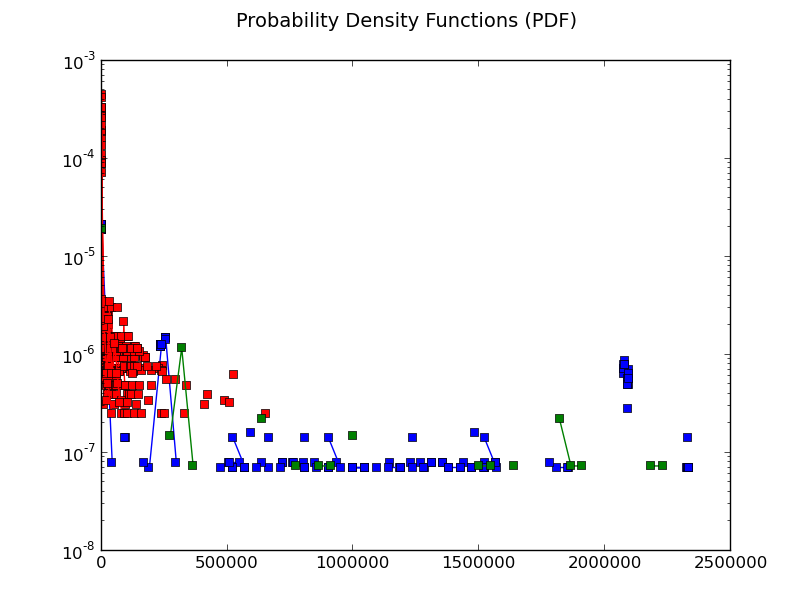
\includegraphics[width=\textwidth]{pdf_cdf/pdf.png}
    \caption{Probability Density Functions (PDF)}
    \label{fig:pdf}
  \end{minipage}
  \hfill
  \begin{minipage}[b]{0.4\textwidth}
    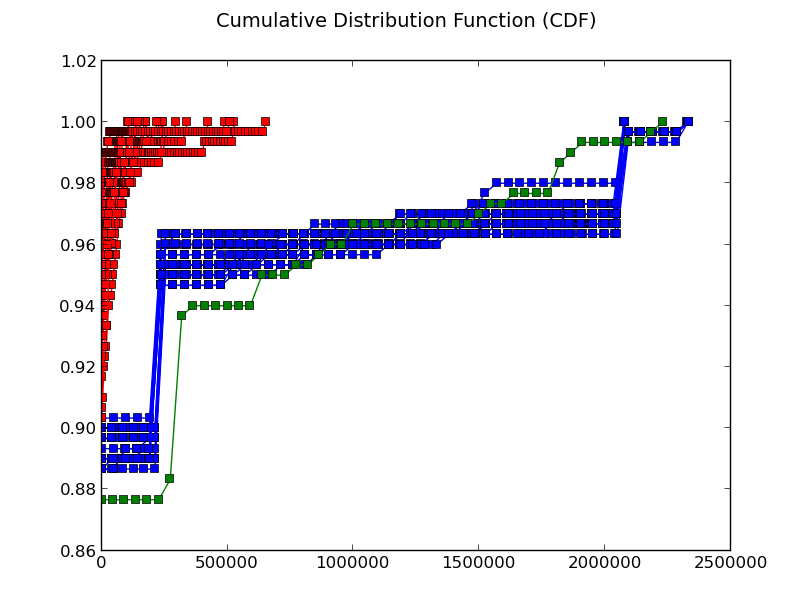
\includegraphics[width=\textwidth]{pdf_cdf/cdf.png}
    \caption{Cumulative Distribution Function (CDF)}
    \label{fig:cdf}
  \end{minipage}
\end{figure}

Como se pode observar nas figuras \ref{fig:pdf} e \ref{fig:cdf}, nos gráficos, as PDF dos serviços 0 - 19 são representados pela cor azul, e as 20 - 39 são representadas com a cor vermelha. 

Os serviços 0 - 19 estão mais distribuídos pelo eixo dos XX, ou seja, existe mais probabilidade de existir a receção de pacotes com mais frequência.

Os serviços 20 - 39, já existe grande probabilidade de obter zero pacotes, devido aos longos períodos de tempo sem receção de pacotes. 

Devido a esta situação, dos serviços 20-39, os valores de kurtosis e skewness são mais elevados, como se pode ver na figura \ref{fig:compare_profile}.

\newpage
\subsection{Exercício 5}
\subsubsection{codeFiles/qq\_pp\_plot.py (linha 39)}


\begin{figure}[!htb]
  \centering
  \begin{minipage}[b]{0.4\textwidth}
    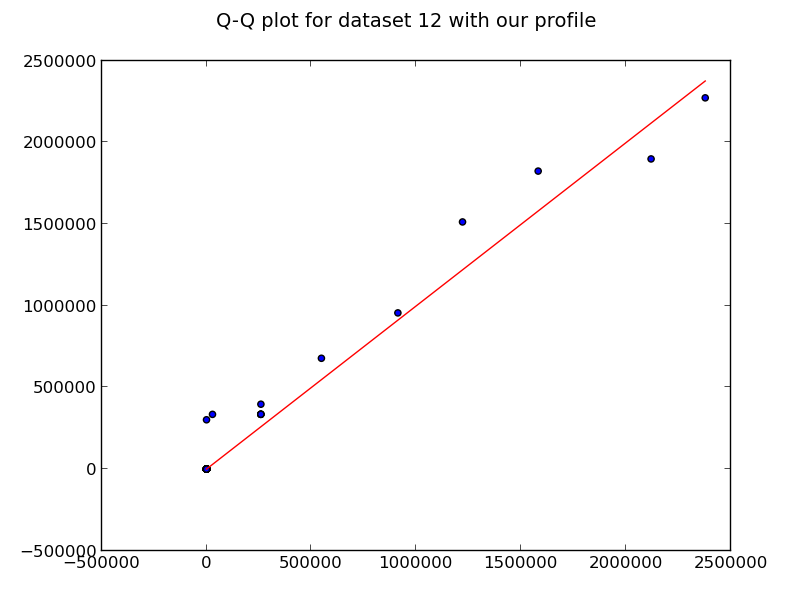
\includegraphics[width=\textwidth]{qq_pp/qq_plot_12.png}
    \caption{Q-Q plot do dataset 12}
    \label{fig:qq_12}
  \end{minipage}
  \hfill
  \begin{minipage}[b]{0.4\textwidth}
    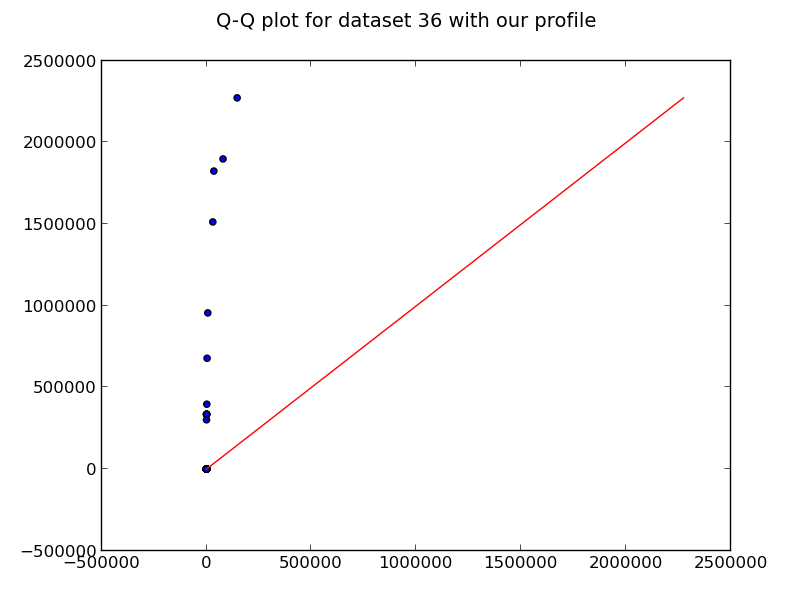
\includegraphics[width=\textwidth]{qq_pp/qq_plot_36.png}
    \caption{Q-Q plot do dataset 36}
    \label{fig:qq_36}
  \end{minipage}
\end{figure}

É possível ver que através da comparação entre o gráfico Q-Q obtido através do serviço 12 com o gráfico Q-Q obtido do serviço 36, o gráfico pertencente ao primeiro grupo (\ref{fig:qq_12}) possui um número de pacotes recebidos maior. O perfil obtido através do YouTube, como já tinha sido verificado acima, enquadra-se neste grupo, e é possível observar esse acontecimento pelos pontos que se encontram muito próximos da linha vermelha, ao contrário do serviço 36.

\newpage
\begin{figure}[!htb]
  \centering
  \begin{minipage}[b]{0.4\textwidth}
    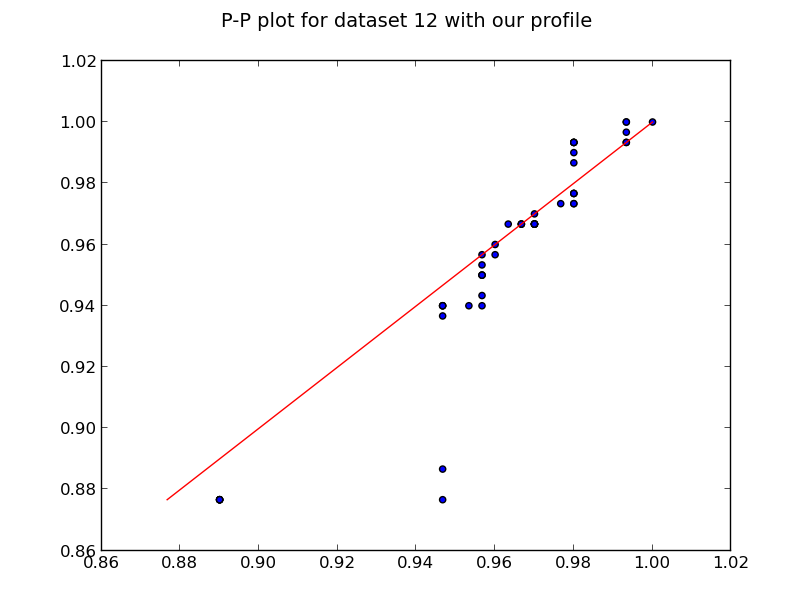
\includegraphics[width=\textwidth]{qq_pp/pp_plot_12.png}
    \caption{P-P plot do dataset 12}
    \label{fig:pp_12}
  \end{minipage}
  \hfill
  \begin{minipage}[b]{0.4\textwidth}
    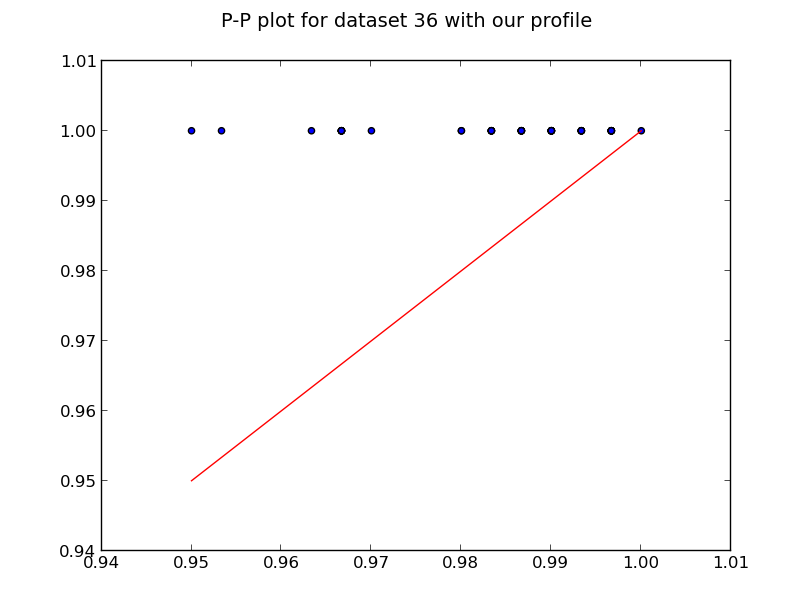
\includegraphics[width=\textwidth]{qq_pp/pp_plot_36.png}
    \caption{P-P plot do dataset 36}
    \label{fig:pp_36}
  \end{minipage}
\end{figure}

O P-P plot, consiste no confronto entre duas distribuições cumulativas (CDF's) de dois perfis, neste caso, entre o perfil do dataset 12 e 36 com o perfil do YouTube. É possível verificar que tal como nas CDF's dos serviços entre 20 e 39 (\ref{fig:cdf}), rapidamente ascende ao valor 1, enquanto que no caso dos serviços entre 0 e 19, onde o perfil YouTube se enquadra, os pontos acompanham a linha, com uma proximidade relativamente baixa, pelo que é possível verificar as conclusões retiradas acima, em relação ao tipo de perfil.

\subsection{Exercício 6}
\subsubsection{codeFiles/pdf\_cdf.py (linha 128)}

\begin{figure}[!htb]
\center
 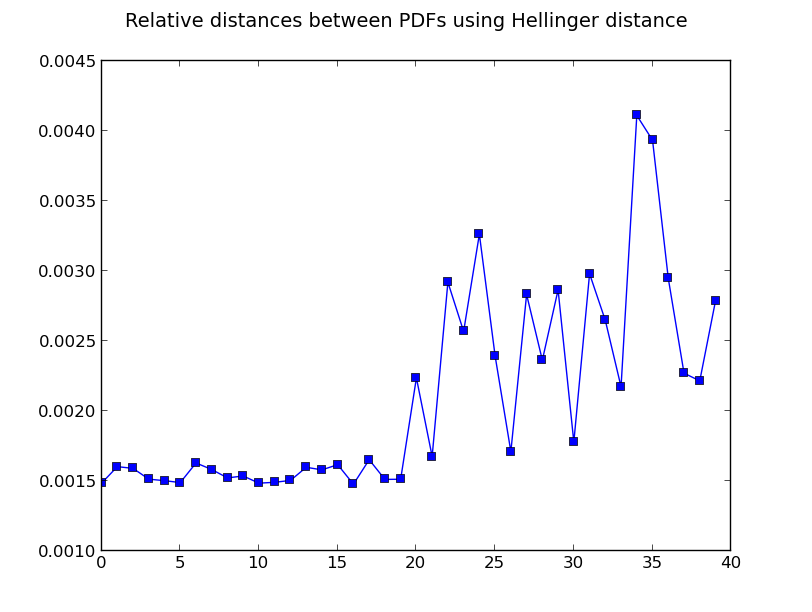
\includegraphics[width=100mm,scale=1]{hellingerDist/Relative_distances_between_PDFs_using_Hellinger_distance_plot.png}
 \caption{Distâncias relativas entre PDF's}
 \label{fig:hellingerDist}
\end{figure}

Através do gráfico de distâncias relativas entre PDF's, utilizando a distância de Hellinger, é possível observar, que entre os primeiros datasets 0-19 e o dataset do YouTube, a distância é relativamente pequena. Já nos datasets 20-39, a distância sofre um aumento bastante significativo, pelo que é possível concluir mais uma vez, que o perfil de YouTube, se enquadra mais nos primeiros 20 datasets.

\subsection{Exercício 7}
\subsubsection{codeFiles/pdf\_cdf.py (linha 135)}

\begin{figure}[!htb]
\center
 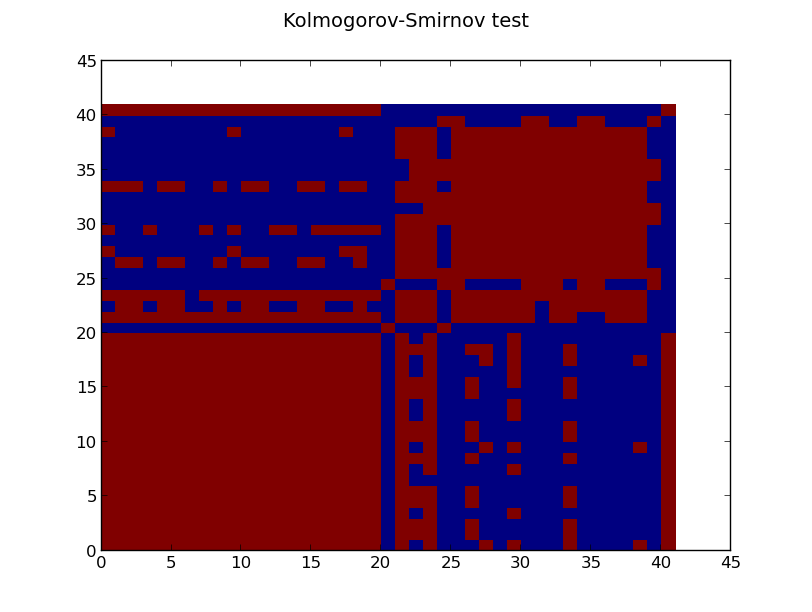
\includegraphics[width=100mm,scale=1]{hellingerDist/Kolmogorov-Smirnov_test.png}
 \caption{Teste de Kolmogorov-Smirnov}
 \label{fig:kolmogorov}
\end{figure}

Neste teste, o objetivo era saber se dois perfis seguiam a mesma distribuição. Através do cálculo de um \textit{p-value}, obtido através de dois datasets. Caso este valor, fosse inferior ao nível de significância (neste caso 5\%), a hipótese de os dois perfis seguirem a mesma distribuição era rejeitada. É possível verificar na imagem acima (\ref{fig:kolmogorov} que nos datasets pertencentes ao mesmo grupo, a hipótese é aceite, ficando preenchido a vermelho. Quando pertencem a grupos diferentes, é possível verificar que a maioria das vezes a hipótese é rejeitada (ilustrado a azul).

O perfil obtido do YouTube, na imagem, corresponde ao dataset 40, pelo que é facilmente identificável, que este pertence ao primeiro grupo de perfis.

\newpage
\section{Multivariate Distributions}
\subsection{Exercício 8}
\subsubsection{codeFiles/pdf\_cdf.py (linha 193)}

\begin{figure}[!htb]
  \centering
  \begin{minipage}[b]{0.4\textwidth}
    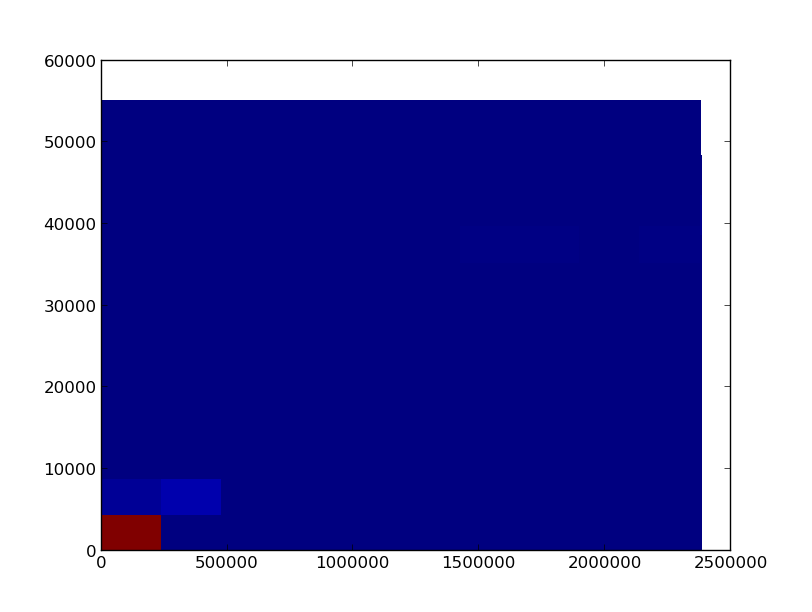
\includegraphics[width=\textwidth]{multivariate_dist/histogram2d_serv_9.png}
    \caption{Histograma 2D, Dataset 9}
    \label{fig:hist_serv9}
  \end{minipage}
  \hfill
  \begin{minipage}[b]{0.4\textwidth}
    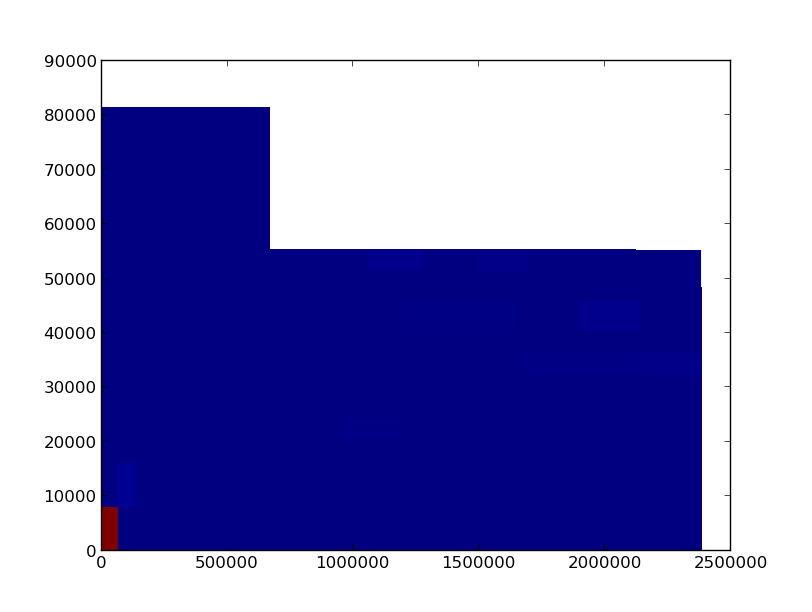
\includegraphics[width=\textwidth]{multivariate_dist/histogram2d_serv_30.png}
    \caption{Histograma 2D, Dataset 30}
    \label{fig:hist_serv30}
  \end{minipage}
\end{figure}

Neste exercício foi pedido para obter as pdf's dos serviços, sendo desta vez utilizadas duas variáveis, upload e download.

Nos gráficos presentes nas figuras \ref{fig:hist_serv9} e \ref{fig:hist_serv30}, são visíveis vários níveis de cor, sendo que os pontos vermelhos correspondem a um valor da probabilidade maior e nos pontos azuis, a probabilidade é mais pequena.

O gráfico obtido do Dataset 9, pertencente ao primeiro grupo de Datasets, permite verificar que junto ao ponto 0, a prababilidade é maior, isto porque, os pacotes são recebidos em bursts, e a maior parte das vezes, não é recebido qualquer pacote. Os bursts, são representados pelos quadrados azul mais claro.

Já no gráfico do Dataset 30, continua a existir uma maior probabilidade junto ao ponto 0, contudo mais próximo do zero do que o anterior e existem ainda menos quadrados azul claro.

Conclui-se que em ambos os serviços, a probabilidade é maior junto ao ponto (0,0). Verifica-se ainda que o upload é muito inferior ao download, e no segundo grupo de datasets é mais superior do que o do primeiro grupo.

\newpage
\section{Aggregation Effect}
\subsection{Exercício 9}
\subsubsection{codeFiles/pdf\_cdf.py (linha 206)}

\begin{figure}[!htb]
  \centering
  \begin{minipage}[b]{0.4\textwidth}
    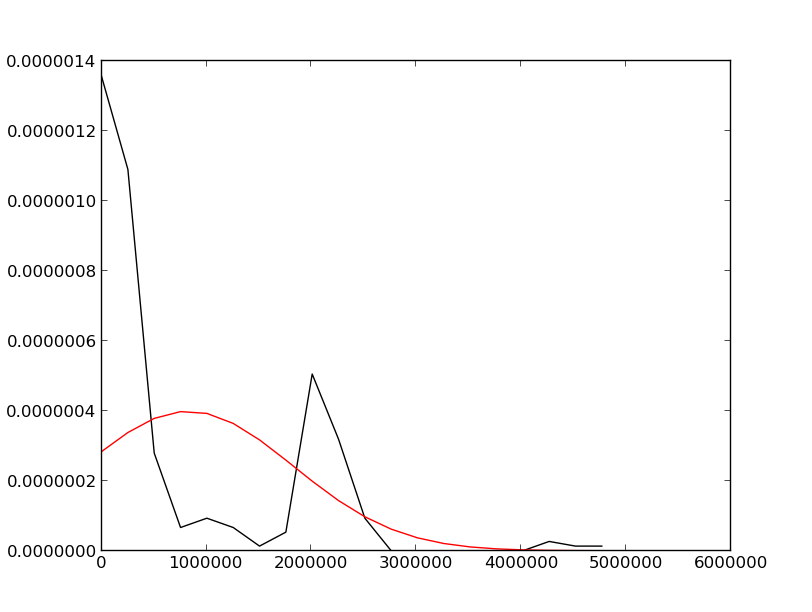
\includegraphics[width=\textwidth]{aggregation_effect/empirical_PDF__20_users_.png}
    \caption{PDF 20 utilizadores}
    \label{fig:empirical_20_users}
  \end{minipage}
  \hfill
  \begin{minipage}[b]{0.4\textwidth}
    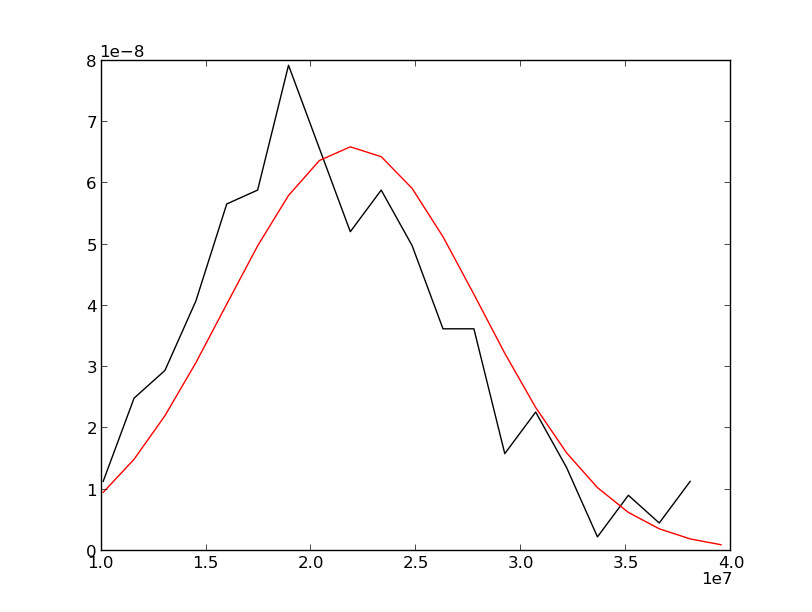
\includegraphics[width=\textwidth]{aggregation_effect/empirical_PDF__500_users_.png}
    \caption{PDF 500 utilizadores}
    \label{fig:empirical_500_users}
  \end{minipage}
\end{figure}

Com este exercício era pretendido verificar que quanto maior o número de utilizadores agregados, maior seria a aproximação à curva Gaussiana. Tal como as imagens (\ref{fig:empirical_20_users}, \ref{fig:empirical_500_users}) demonstram, quando se tem apenas 20 utilizadores, não existe grande aproximação à curva Gaussiana. Quando se tem 500 utilizadores, a aproximação é bastante significativa, tal como pretendido.

\newpage
\section{Events Correlation}
\subsection{Exercício 10}
\subsubsection{codeFiles/pdf\_cdf.py (linha 224)}

\begin{figure}[!htb]
\center
 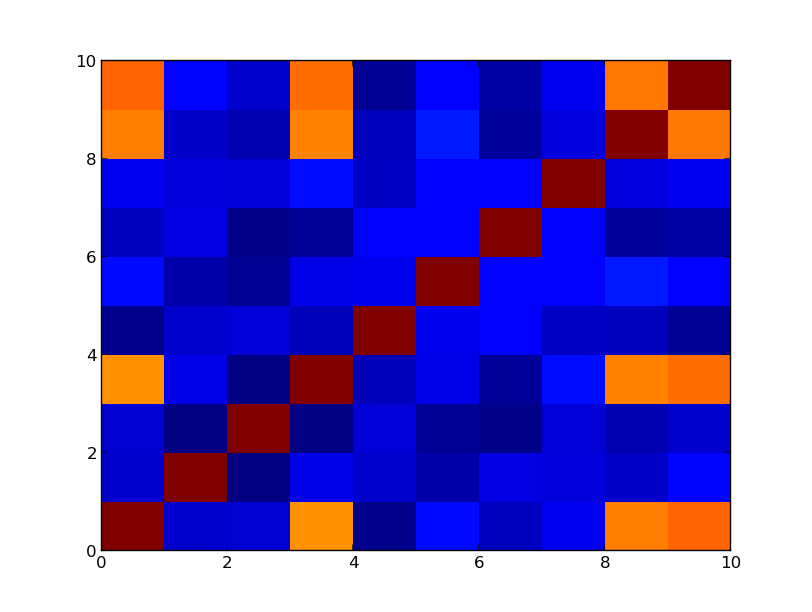
\includegraphics[width=100mm,scale=1]{event_correlation/event_correlation.png}
 \caption{Correlação de eventos}
 \label{fig:event_correlation}
\end{figure}

A anomalia no tráfego existente no link 1 fez com que esta, se propagasse pelos links 4 (coluna 3), 9 (coluna 8) e 10 (coluna 9). Através da figura \ref{fig:event_correlation}, podemos verificar que os links que se encontram a amarelo/laranja, são os que foram afetados pela anomalia do link 1.

\newpage
\section{Periodicity}
\subsection{Exercício 11}
\subsubsection{codeFiles/pdf\_cdf.py (linha 236)}

\begin{figure}[!htb]
  \centering
  \begin{minipage}[b]{0.4\textwidth}
    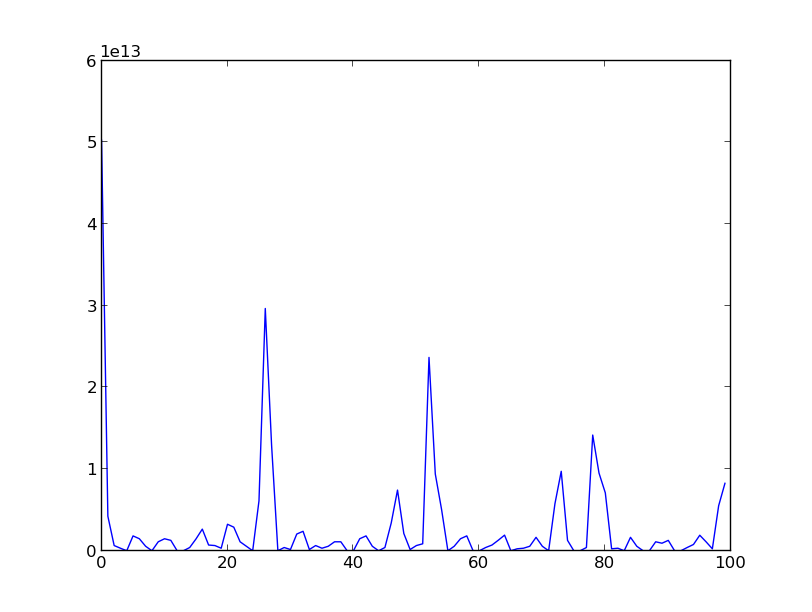
\includegraphics[width=\textwidth]{periodicity/periodicity_service_3.png}
    \caption{Periodicidade Dataset 3}
    \label{fig:periodicity_3}
  \end{minipage}
  \hfill
  \begin{minipage}[b]{0.4\textwidth}
    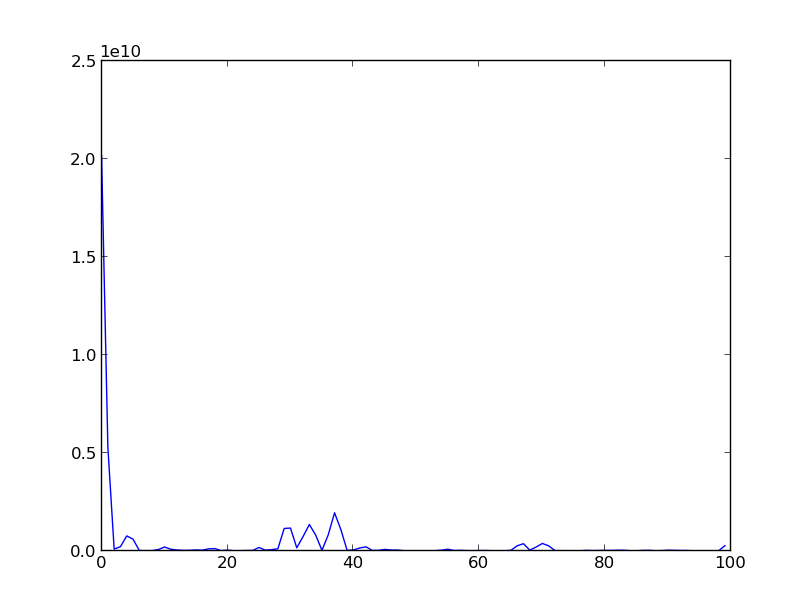
\includegraphics[width=\textwidth]{periodicity/periodicity_service_22.png}
    \caption{Periodicidade Dataset 22}
    \label{fig:periodicity_22}
  \end{minipage}
\end{figure}

Através das figuras \ref{fig:periodicity_3} e \ref{fig:periodicity_22}, é possível verificar que no Dataset 3 existe periodicidade com o decorrer do tempo, sendo neste caso a periodicidade aproximadamente de 26. No outro caso, Dataset 22, verifica-se que não existe periodicidade.

\subsection{Exercício 12}
\subsubsection{codeFiles/pdf\_cdf.py (linha 258)}

\begin{figure}[!htb]
  \centering
  \begin{minipage}[b]{0.4\textwidth}
    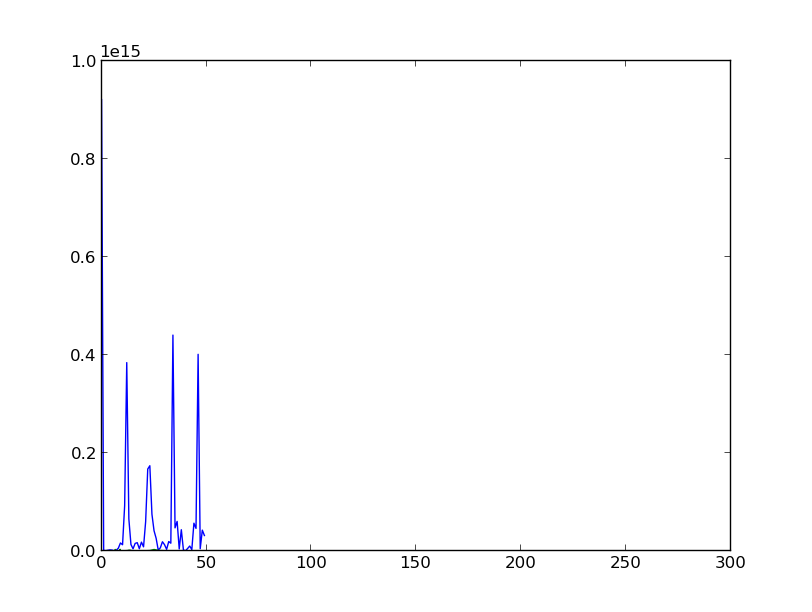
\includegraphics[width=\textwidth]{periodogram/periodogram3.png}
    \caption{Periodogram Dataset 3}
    \label{fig:periodogram_3}
  \end{minipage}
  \hfill
  \begin{minipage}[b]{0.4\textwidth}
    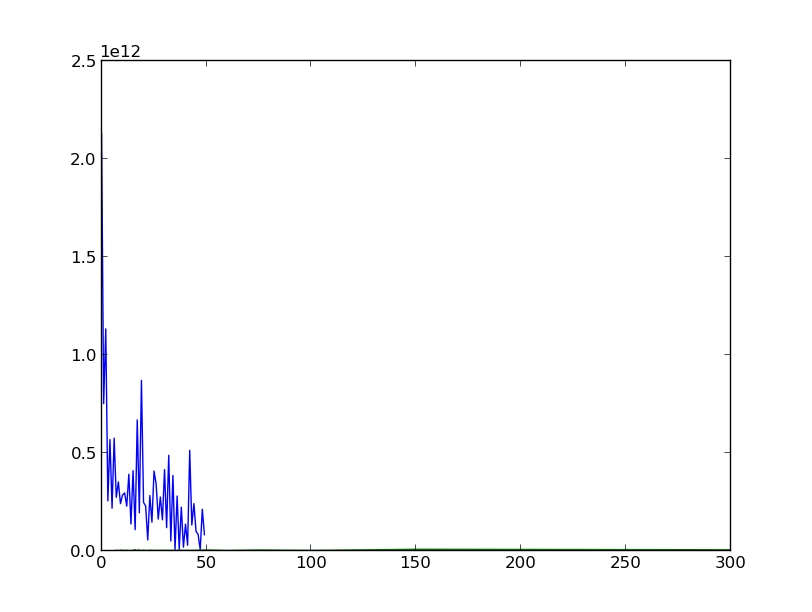
\includegraphics[width=\textwidth]{periodogram/periodogram27.png}
    \caption{Periodogram Dataset 22}
    \label{fig:periodogram_27}
  \end{minipage}
\end{figure}

Através dos periodograms \ref{fig:periodogram_3} e \ref{fig:periodogram_27}, é possível verificar o mesmo que no exercício anterior, existindo uma periodicidade nos datasets pertencentes ao primeiro grupo.
\newpage
\subsection{Exercício 13}
\subsubsection{codeFiles/pdf\_cdf.py (linha 278)}

\begin{figure}[!htb]
  \centering
  \begin{minipage}[b]{0.4\textwidth}
    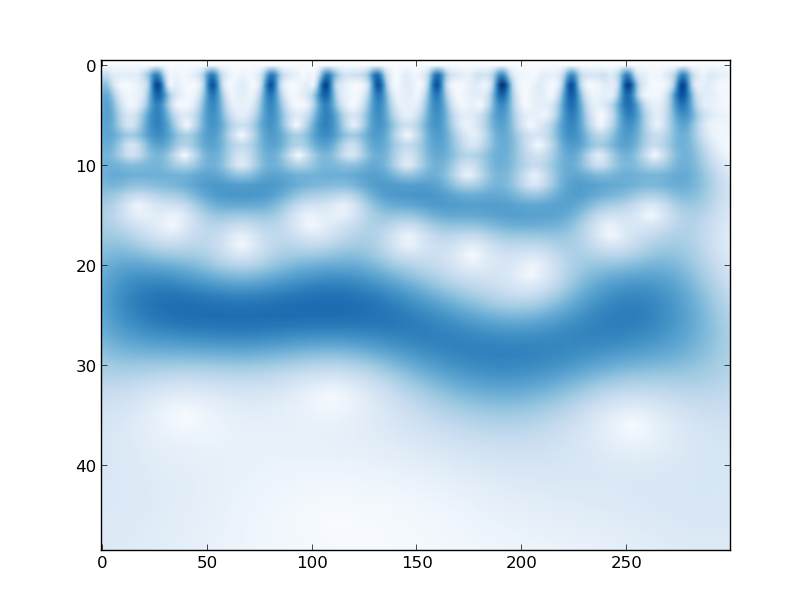
\includegraphics[width=\textwidth]{scalogram/scalogramfft2.png}
    \caption{Scalogram FFT Dataset 2}
    \label{fig:scalogramfft2}
  \end{minipage}
  \hfill
  \begin{minipage}[b]{0.4\textwidth}
    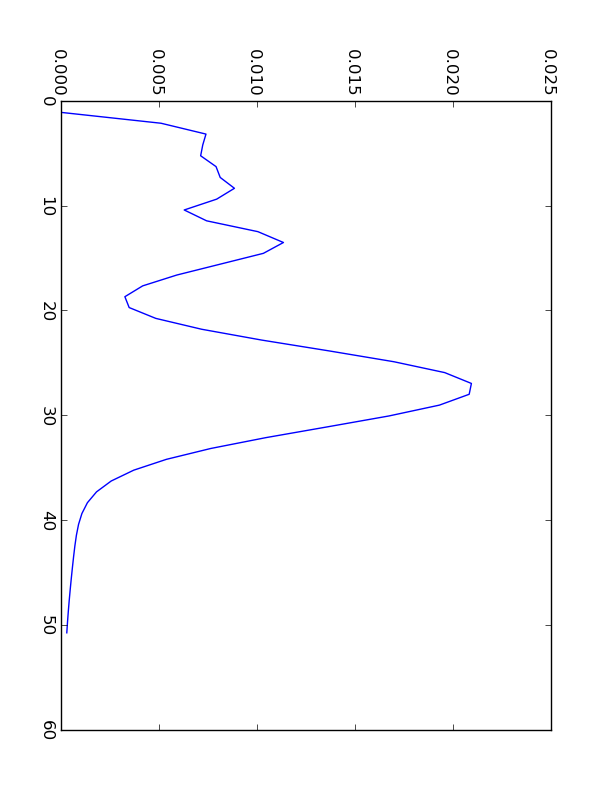
\includegraphics[width=\textwidth]{scalogram/scalogramCWT2.png}
    \caption{Scalogram Dataset 2}
    \label{fig:scalogram2}
  \end{minipage}
\end{figure}

Nas imagens acima, foi feito o Scalogram para um dataset do primeiro grupo de serviços, sendo possível observar que nas zonas mais escuras é um pico de frequência com mais intensidade, podendo perceber-se facilmente a existência de periodicidade.

\newpage
\begin{figure}[!htb]
  \centering
  \begin{minipage}[b]{0.4\textwidth}
    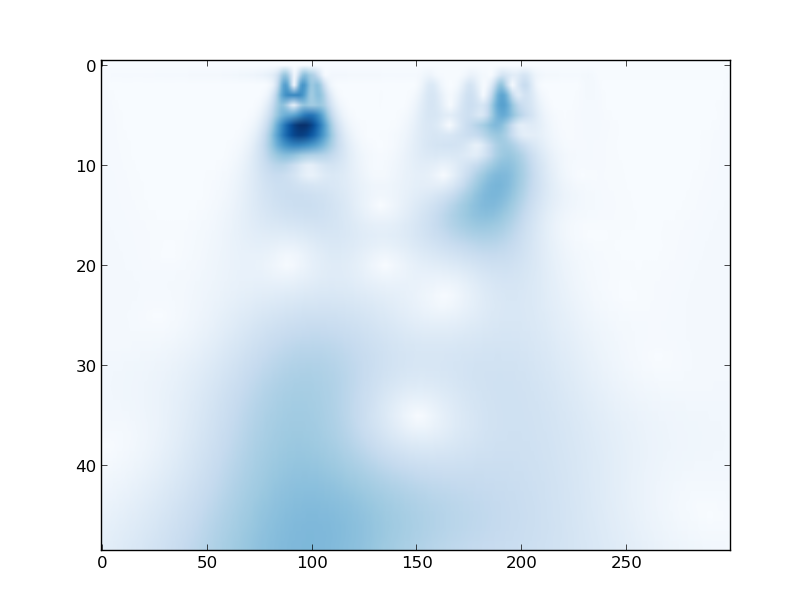
\includegraphics[width=\textwidth]{scalogram/scalogramfft31.png}
    \caption{Scalogram FFT Dataset 31}
    \label{fig:scalogramfft31}
  \end{minipage}
  \hfill
  \begin{minipage}[b]{0.4\textwidth}
    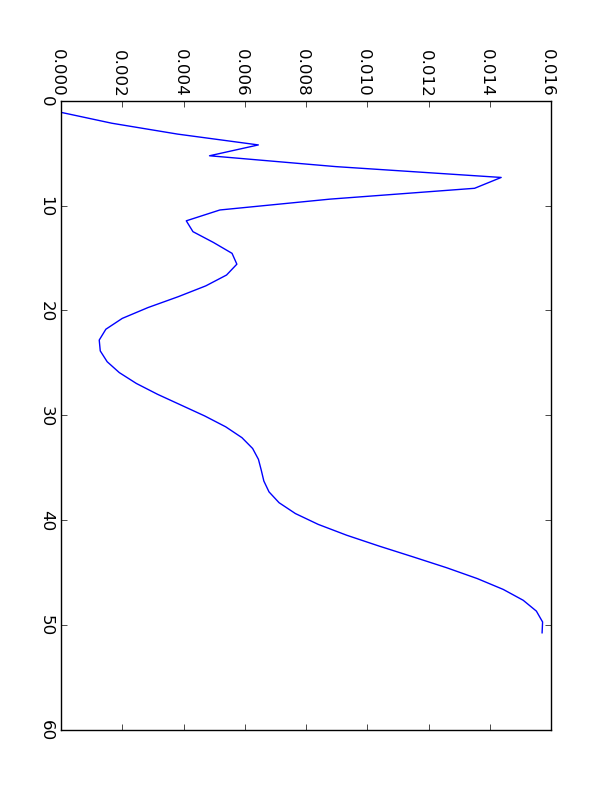
\includegraphics[width=\textwidth]{scalogram/scalogramCWT31.png}
    \caption{Scalogram Dataset 31}
    \label{fig:scalogram31}
  \end{minipage}
\end{figure}

Posteriormente, obteve-se o Scalogram para um dataset do segundo grupo, e obteve-se um valor idêntico mas a periodicidade não é tão evidente como no exemplo anterior.

\newpage
\section{Variable Reduction}
\subsection{Exercício 14}
\subsubsection{codeFiles/classifier.py (linha 58)}

\begin{figure}[!htb]
\center
 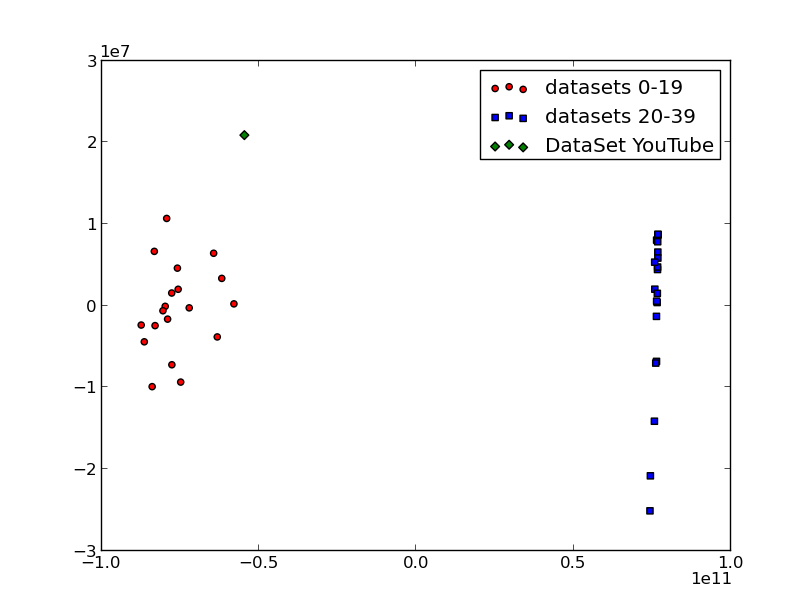
\includegraphics[width=100mm,scale=1]{classifier/PCA.png}
 \caption{PCA}
 \label{fig:pca}
\end{figure}

Utilizando PCA reduzimos variáveis como a média, a mediana, variância, skewness, kurtosis, entre outros, a componentes principais. É possível então através da imagem acima, que o perfil obtido do YouTube, encontra-se de acordo com os perfis do primeiro grupo de perfis. É então feito um fit, com todas as variáveis, seguindo de uma transformação, sendo a diferenciação de perfis, feita com as métricas transformadas e não com as variáveis de média, etc.
Quando já existe uma transformação, todas as métricas que chegarem, podem ser transformadas sem ser feito o fit.
A tranformação origina pontos x, y e alfa1, alfa2, que são utilizados para preencher o gráfico.
\newpage
\subsection{Exercício 15}
\subsubsection{codeFiles/classifier.py (linha 106)}

\begin{figure}[!htb]
\center
 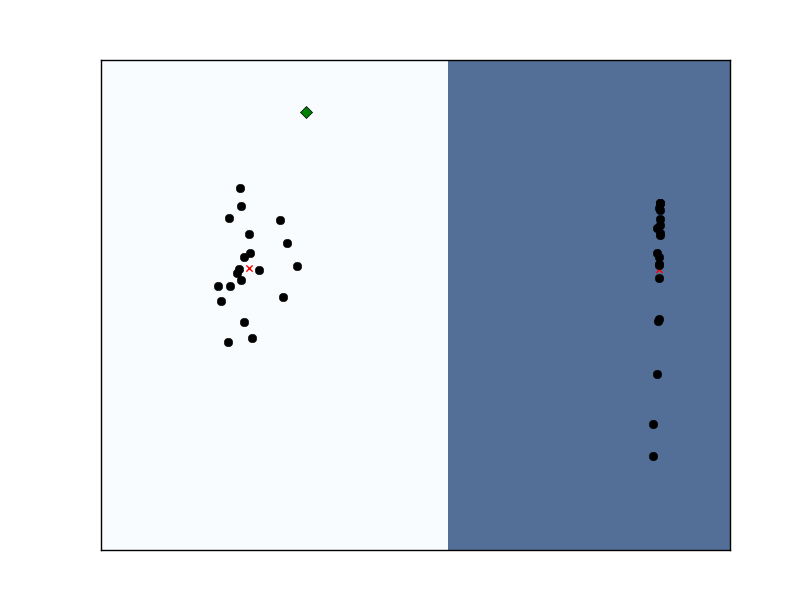
\includegraphics[width=100mm,scale=1]{classifier/K_means.png}
 \caption{K-Means}
 \label{fig:k_means}
\end{figure}

Neste exercício, pretende-se diferenciar utilizadores, desta feita, utilizando o método K-means, que requer um conhecimento à priori do número de clusters existentes. É então feito o fit das componentes, que serve para definir/criar grupos de utilizadores. Posto isto é feito o predict, que vai receber os dados e classificá-los. É possível ver na imagem \ref{fig:k_means}, um gráfico de pontos idêntico ao PCA, sendo que neste a divisão dos grupos é mais clara, sendo feita através das cores branco e azul, sendo os pontos da parte branca pertencentes aos datasets 0-19 e os da zona azul pertencentes aos datasets 20-39. 

O perfil do YouTube, como esperado encontra-se junto aos pontos do primeiro grupo de utilizadores.

\newpage
\subsection{Exercício 16}
\subsubsection{codeFiles/classifier.py (linha 157)}

\begin{figure}[!htb]
\center
 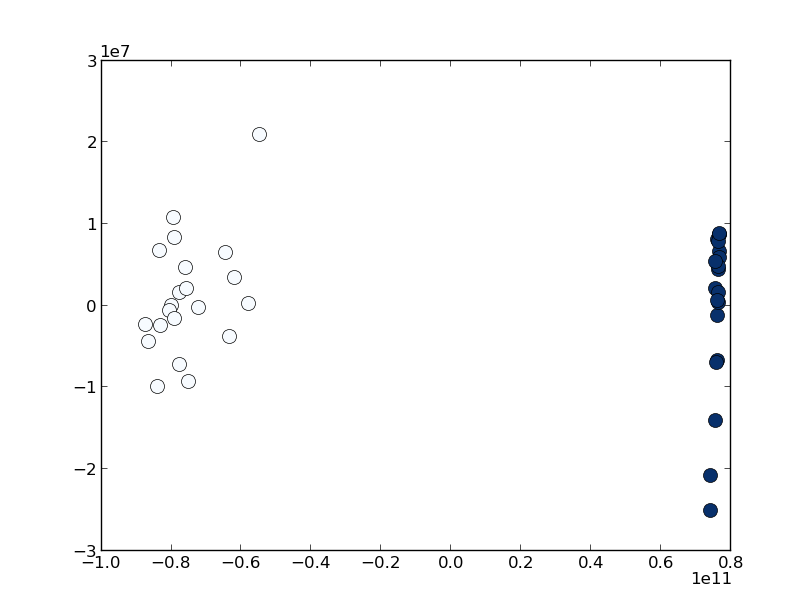
\includegraphics[width=100mm,scale=1]{classifier/DBSCAN.png}
 \caption{DBSCAN}
 \label{fig:dbscan}
\end{figure}

Um outro método para fazer a diferenciação de utilizadores é o DBSCAN, neste não existe número de clusters. Este método baseia-se nas distâncias relativas, sendo com isto necessário correr sempre o fit, quando recebe algo novo.

O perfil do YouTube, foi colocado no grupo dos datasets 0-19, contudo, o esperado, segundo o professor seria a criação de um novo grupo, onde estaria o perfil, mas esta criação de grupo depende da largura de banda com que se obteve os dados, pelo que no nosso caso, não houve a criação de um grupo.

\newpage
\section{Anomaly Identification}
\subsection{Exercício 17}
\subsubsection{codeFiles/classifier.py (linha 177)}

\begin{figure}[!htb]
  \centering
  \begin{minipage}[b]{0.4\textwidth}
    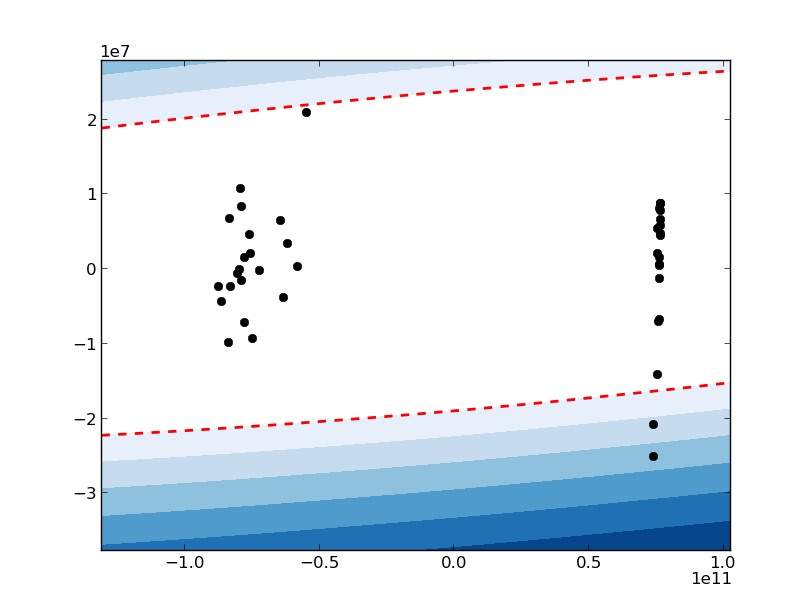
\includegraphics[width=\textwidth]{anomaly/ex17_4_5.png}
    \caption{Assumindo que existem 4.5\% de anomalias}
    \label{fig:anomaly4_5}
  \end{minipage}
  \hfill
  \begin{minipage}[b]{0.4\textwidth}
    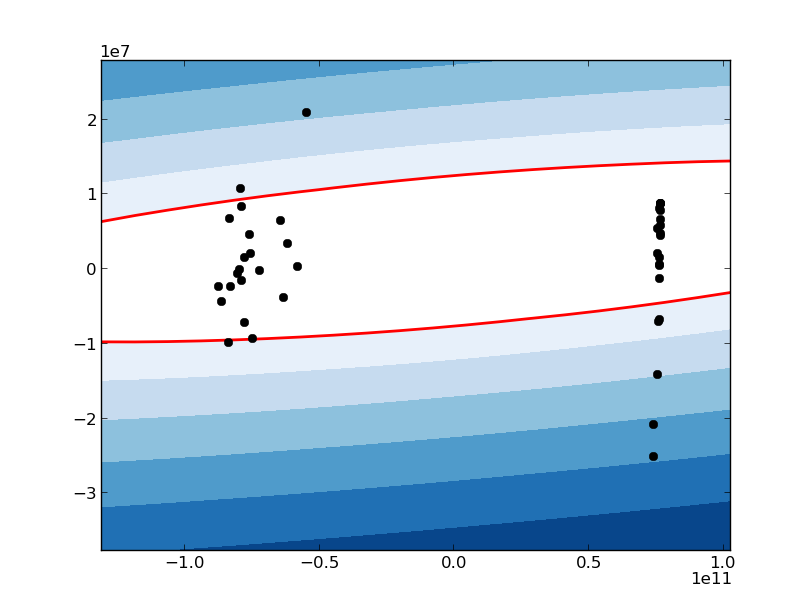
\includegraphics[width=\textwidth]{anomaly/ex17_20.png}
    \caption{Assumindo que existem 20\% de anomalias}
    \label{fig:anomaly20}
  \end{minipage}
\end{figure}

É possível através das figuras \ref{fig:anomaly4_5} e \ref{fig:anomaly20} verificar num conjunto de utilizadores, os que são considerados anomalias. Para isso, são definidas fronteiras, sendo que tudo o que se encontre fora das mesmas, é considerado anomalia. Neste caso, na figura \ref{fig:anomaly4_5}, assumiu-se uma percentagem de anomalias de 4.5\%, tornando o intervalo da fronteira maior, sendo que serão menos os casos de anomalia. Na figura \ref{fig:anomaly20}, assumiu-se uma percentagem de 20\% de anomalias, pelo que o intervalo é mais reduzido, e são então, detetadas mais anomalias.

Contudo, esta experiência, deveria ser feita em grupos, de forma a detetar as anomalias dentro de um determinado grupo, e não no conjunto total de utilizadores, onde os perfis dos utilizadores do primeiro grupo, são anomalias do segundo grupo, e vice-versa.

\newpage
\section{Single Distribution Models}
\subsection{Exercício 18}
\subsubsection{codeFiles/distribution.py (linha 19)}

\begin{figure}[!htb]
\center
 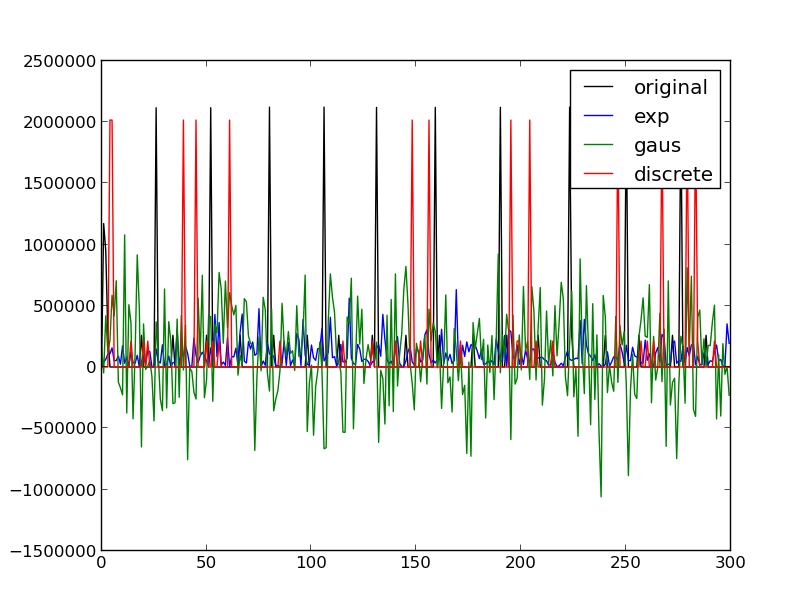
\includegraphics[width=100mm,scale=1]{distribution/ex18.png}
 \caption{Distribuição original, exponencial, gaussiana e discreta}
 \label{fig:ex18}
\end{figure}

Neste exercício, era pedido, para através de um perfil qualquer, tentar arranjar uma distribuição que descrevesse o comportamento do mesmo. Era pedido que se ajustasse a distribuição de forma exponencial, normal e discreta, de forma a se comparar com as PDF's do perfil original.

Para gerar a distribuição de forma exponencial apenas era necessária a média dos valores da distribuição original. No caso de gerar uma distribuição normal/gaussiana, seria necessária, para além da média dos valores, a variância.

Neste exercício, apenas se olha para quantidade e não para tempo, pelo que não é possível ter uma noção exata de periodicidade, existe uma discrepância na mesma.

\newpage

\section{Machine State Modulated Distributions}
\subsection{Exercício 19}
\subsubsection{codeFiles/distribution.py (linha 47)}


No exercício 19, era pedido que se criasse um gerador de perfis através de um gráfico ON/OFF, que consiste numa máquina de dois estados, que saltam de um para o outro. Quando se encontra no estado ON, gera pacotes com uma taxa lambda. 

É definida uma fronteira, que no neste caso foi com o valor de 1, em que tudo o que se encontra acima encontra-se no estado ON, o resto encontra-se no estado OFF.

\begin{figure}[!htb]
\center
 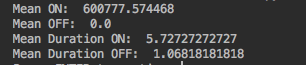
\includegraphics[width=100mm,scale=1]{distribution/ex19Terminal.png}
 \caption{Médias ON/OFF e Médias Duração ON/OFF}
 \label{fig:ex19Terminal}
\end{figure}

O perfil que se estudou, para uma fronteira com o valor de 1, tinha de médias, como se pode ver na figura acima, 600777.574468 para o estado ON e 0.0 para o estado OFF, o que é o esperado, pois o estado OFF é quando não gera praticamente pacotes nenhuns.

Em relação ao tempo médio que se encontra em cada estado, é possível verificar que se encontra mais no estado OFF, com uma média de 5.727, do que no estado ON, que tem uma média de 1.06818.

\begin{figure}[!htb]
\center
 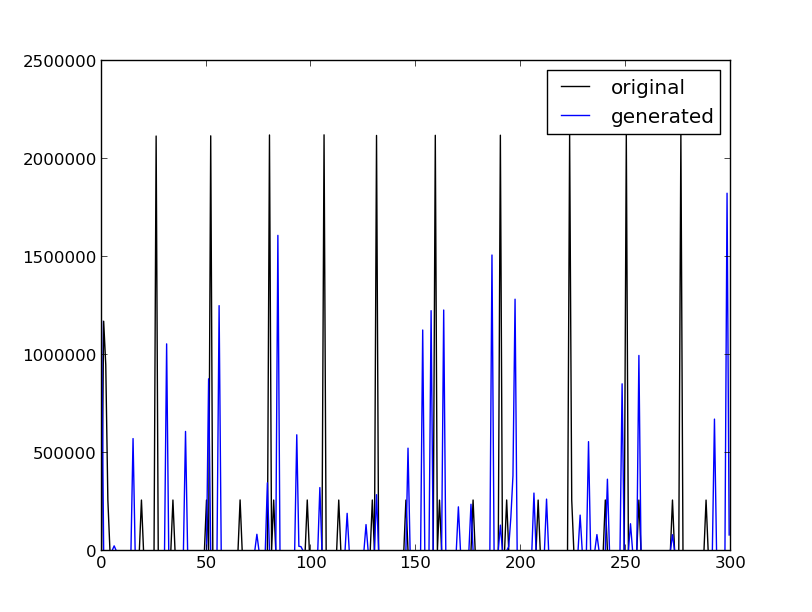
\includegraphics[width=100mm,scale=1]{distribution/ex19.png}
 \caption{Distribuição do perfil original e do gerado}
 \label{fig:ex19}
\end{figure}

Depois da obtenção das médias, gerou-se um novo perfil que seguiria a mesma distribuição, sendo possível verificar, através do gráfico apresentado na figura \ref{fig:ex19}, que o objetivo foi conseguido, pelo que o novo perfil se enquadra na distribuição desejada, com picos como o original, mas na maioria das vezes com pouca produção de pacotes.

\newpage
\section{Trend/Growth Models}
\subsection{Exercício 20}
\subsubsection{codeFiles/distribution.py (linha 103)}

\begin{figure}[!htb]
\center
 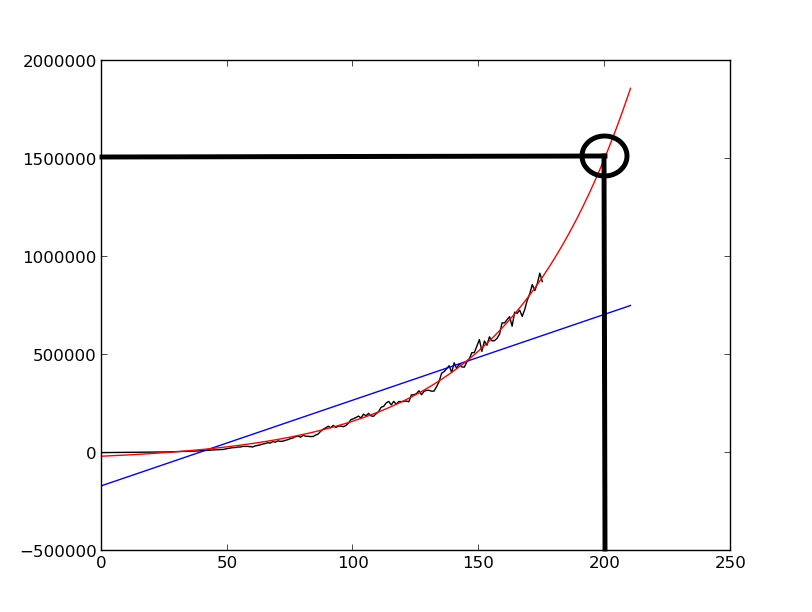
\includegraphics[width=100mm,scale=1]{distribution/ex20.png}
 \caption{Distribuição original, exponencial, gaussiana e discreta}
 \label{fig:ex18}
\end{figure}

O objetivo deste último exercício, era prever o tempo que demorará o tráfego de entrada no IX em Amsterdão a atingir 1.5 ExaBytes.
Sabendo, que no momento da captura que permitiu a elaboração do gráfico, o tempo ia em 180 meses (fim da linha preta), através do gráfico é possível ver que o valor de tráfego será atingido no mês 200, pelo que em 20 meses o tráfego de entrada, já terá atingido valores nos 1.5 ExaBytes.

É possível ainda verificar através da curva a vermelho, que cada vez mais a subida de valores no tráfego é mais rápida pelo que demorará menos tempo a atingir valores ainda mais elevados.

A curva a vermelho, foi encontrada com um ajuste exponencial, de forma a se aproximar com a realidade, e é possível verificar que está enquadrada com a curva real (linha preta).

\end{document}

